\documentclass[acmtog, anonymous, review]{acmart}
\acmSubmissionID{228}

\usepackage{booktabs} % For formal tables
\usepackage{amssymb}
\usepackage{graphicx}
\graphicspath{{/home/guoyu/Dropbox/Bayesian_appearance/}{/home/milos/Dropbox/Bayesian_appearance/}{/Users/shuangz/Dropbox/Bayesian_appearance/}}
\usepackage{xspace}
\usepackage{paralist}
\usepackage{bm}       %provides boldmath symbols via \bm command
\usepackage{accents}
\usepackage{relsize}      %provides easy changing of text size including in mathmode
% \usepackage{subfigure}
\usepackage{subcaption}
\usepackage{caption}
\usepackage{overpic}
\usepackage{makecell}
\usepackage{multirow}
\usepackage{float}


% Copyright
% \setcopyright{none}
%\setcopyright{acmcopyright}
%\setcopyright{acmlicensed}
%\setcopyright{rightsretained}
%\setcopyright{usgov}
%\setcopyright{usgovmixed}
%\setcopyright{cagov}
%\setcopyright{cagovmixed}


% DOI
% \acmDOI{10.475/123_4}

% ISBN
% \acmISBN{123-4567-24-567/08/06}

% Conference
\acmConference[SIGGRAPH 2019]{SIGGRAPH 2019}{July 2019}{Los Angeles}
\acmYear{2019}
\copyrightyear{2019}

% \acmPrice{15.00}

\citestyle{acmauthoryear}
\setcitestyle{square}

\usepackage{amsmath}
\DeclareMathOperator*{\argmin}{arg\,min}
\DeclareMathOperator*{\argmax}{arg\,max}
\usepackage{amssymb}
\usepackage{booktabs} % For formal tables
\usepackage{xspace}
\usepackage{paralist}
\usepackage{bm}       %provides boldmath symbols via \bm command
%\usepackage{accents}
\usepackage{relsize}      %provides easy changing of text size including in mathmode
\usepackage{subcaption}
\usepackage{caption}
\usepackage{overpic}
\usepackage{makecell}
\usepackage{multirow}
\usepackage{float}
\graphicspath{{D:/gyDocuments/Dropbox/Bayesian_appearance/}{/home/guoyu/Dropbox/Bayesian_appearance/}{/Users/mihasan/Dropbox/Bayesian_appearance/}{/Users/shuangz/Dropbox/Bayesian_appearance/}}

\newcommand{\Reals}{\mathbb{R}}
\newcommand{\summ}{\mathbb{S}}
\newcommand{\la}{\leftarrow}
\newcommand{\ra}{\rightarrow}
\newcommand{\lra}{\leftrightarrow}
\newcommand{\bd}{\bm{d}}
\newcommand{\bz}{\bm{z}}
\newcommand{\btheta}{\bm{\theta}}
\newcommand{\target}{\bm{I}_t}
\newcommand{\synth}{\bm{I}_s}
\newcommand{\bsigma}{\bm{\Sigma}}
\newcommand{\fsigma}{\sigma_f}
\newcommand{\fsigmax}{\sigma_{fx}}
\newcommand{\fsigmay}{\sigma_{fy}}
\newcommand{\fscale}{c_f}
\newcommand{\light}{E}
\newcommand{\bx}{\bm{x}}
\newcommand{\by}{\bm{y}}
\newcommand{\bom}{\bm{\omega}}
\newcommand{\pc}{\alpha}

\newcommand{\milos}[1]{\textcolor{blue}{[\textbf{Milos:} {\em #1}]}}
\newcommand{\fixme}[1]{\textcolor{red}{[\textbf{FIXME:} {\em #1}]}}
\newcommand{\sz}[1]{\textcolor{green}{[\textbf{SZ:} {\em #1}]}}
\newcommand{\gy}[1]{\textcolor{red}{[\textbf{Yu:} {\em #1}]}}
\newcommand{\revision}[1]{\textcolor{blue}{#1}}
\newcommand{\toptext}[2]{$\overbrace{\hspace{#1}}^{\text{\normalsize #2}}$}

\newlength{\resultwidth}
\setlength{\resultwidth}{0.8in}
\newlength{\resultwidthpdf}
\setlength{\resultwidthpdf}{0.7in}

\newcommand{\imglabel}[1]{\put(2,5){\small\bfseries\contour{black}{\textcolor{white}{#1}}}}


%Fix for error when hyperreferences get split across a page boundary
%\hypersetup{draft}

% Alter some LaTeX defaults for better treatment of figures:
% See p.105 of "TeX Unbound" for suggested values.
% See pp. 199-200 of Lamport's "LaTeX" book for details.
%   General parameters, for ALL pages:
\renewcommand{\topfraction}{0.9}	% max fraction of floats at top
\renewcommand{\bottomfraction}{0.8}	% max fraction of floats at bottom
%   Parameters for TEXT pages (not float pages):
\setcounter{topnumber}{2}
\setcounter{bottomnumber}{2}
\setcounter{totalnumber}{4}     % 2 may work better
\setcounter{dbltopnumber}{2}    % for 2-column pages
\renewcommand{\dbltopfraction}{0.99}	% fit big float above 2-col. text
\renewcommand{\textfraction}{0.01}	% allow minimal text w. figs
%   Parameters for FLOAT pages (not text pages):
\renewcommand{\floatpagefraction}{0.7}	% require fuller float pages
% N.B.: floatpagefraction MUST be less than topfraction !!
\renewcommand{\dblfloatpagefraction}{0.7}	% require fuller float pages


\begin{document}
\setcopyright{acmlicensed}
\acmJournal{TOG}
\acmYear{2019}\acmVolume{37}\acmNumber{4}\acmArticle{75}\acmMonth{8} \acmDOI{10.1145/xxxxxxx.xxxxxxx}

\title{A Bayesian Inference Framework for Material Parameter Estimation}
% \titlenote{Produces the permission block, and copyright information}
%\subtitle{Extended Abstract}
% \subtitlenote{The full version of the author's guide is available as \texttt{acmart.pdf} document}


%\author{Yu Guo}
%\affiliation{%
%  %\department{Department of Computer Science}
%  \institution{University of California, Irvine}}
%\email{guo.yu@uci.edu}
%
%\author{Ling-Qi Yan}
%\affiliation{%
%  \institution{University of California, Santa Barbara}
%}
%\email{lingqi@berkeley.edu}
%
%\author{Milo\v s Ha\v san}
%\affiliation{%
%  \institution{Adobe}
%}
%\email{milos.hasan@gmail.com}
%
%\author{Shuang Zhao}
%\affiliation{%
%  \institution{University of California, Irvine}}
%\email{shz@ics.uci.edu}

% % The default list of authors is too long for headers}
% \renewcommand{\shortauthors}{B. Trovato et al.}


\begin{abstract}
Procedural material models have been gaining traction in many applications thanks to their flexibility, compactness, and easy editability.
We explore the inverse rendering problem of procedural material parameter estimation from photographs, presenting a unified view of the problem in a Bayesian framework.
In addition to computing point estimates of the parameters by optimization, our framework uses a Markov Chain Monte Carlo approach to sample the space of plausible material parameters, providing a collection of plausible matches that a user can choose from, and efficiently handling both discrete and continuous model parameters.
To demonstrate the effectiveness of our framework, we fit procedural models of a range of materials---wall plaster, leather, wood, anisotropic brushed metals and layered metallic paints---to both synthetic and real target images.

\end{abstract}

%CCS
\begin{CCSXML}
<ccs2012>
<concept>
<concept_id>10010147.10010371.10010372</concept_id>
<concept_desc>Computing methodologies~Rendering</concept_desc>
<concept_significance>500</concept_significance>
</concept>
% <concept>
% <concept_id>10010147.10010371.10010372.10010374</concept_id>
% <concept_desc>Computing methodologies~Ray tracing</concept_desc>
% <concept_significance>500</concept_significance>
% </concept>
</ccs2012>
\end{CCSXML}

\ccsdesc[500]{Computing methodologies~Rendering}
% \ccsdesc[500]{Computing methodologies~Ray tracing}


\setcopyright{acmlicensed}
\acmJournal{TOG}
\acmYear{2019}\acmVolume{37}\acmNumber{4}\acmArticle{75}\acmMonth{8} \acmDOI{10.1145/xxxxxxx.xxxxxxx}

\keywords{material appearance, Bayesian inference, inverse problems}


\teaser{
	\centering
	\vspace{-1cm}
	\addtolength{\tabcolsep}{-4.5pt}
	\newlength{\insetLen}
	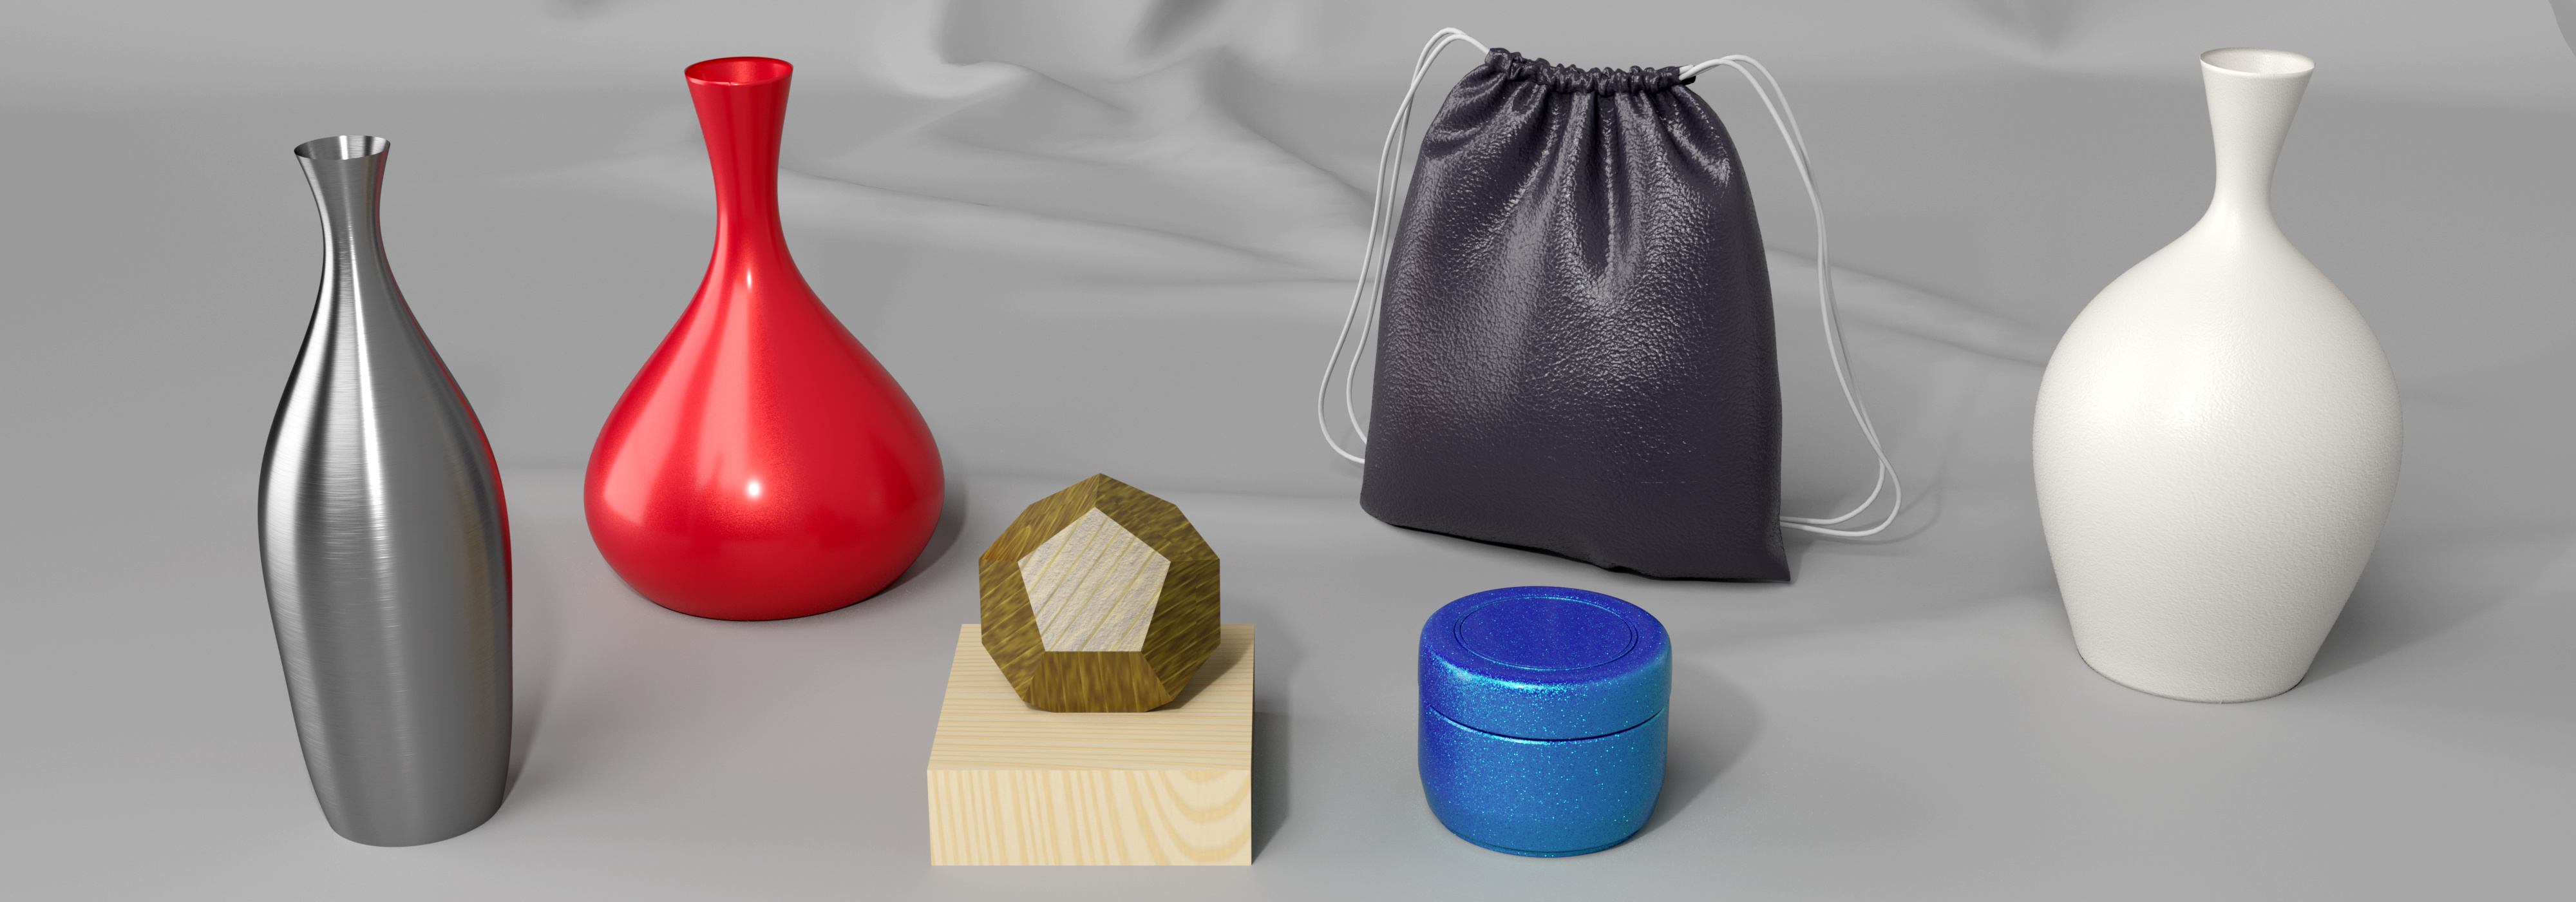
\includegraphics[width=0.98\textwidth]{fig1-2/teaser.jpg}\\[2pt]
	\setlength{\insetLen}{0.132\textwidth}
	\begin{tabular}{cccccccc}
		\raisebox{7pt}{\rotatebox{90}{\small \bfseries Input}} &
		\adjincludegraphics[width=\insetLen,trim={0 {.2\height} 0 {.2\height}},clip]{fig7/5_metal_3/target.jpg} &
		\adjincludegraphics[width=\insetLen,trim={0 {.2\height} 0 {.2\height}},clip]{fig7/4_flake_4/target.jpg} &
		\adjincludegraphics[width=\insetLen,trim={0 {.2\height} 0 {.2\height}},clip]{fig7/6_wood_4/target.jpg} &
		\adjincludegraphics[width=\insetLen,trim={0 {.2\height} 0 {.2\height}},clip]{fig7/6_wood_5/target.jpg} &
		\adjincludegraphics[width=\insetLen,trim={0 {.2\height} 0 {.2\height}},clip]{fig5/4_flake_1/target.jpg} &
		\adjincludegraphics[width=\insetLen,trim={0 {.2\height} 0 {.2\height}},clip]{fig7/2_leather_3/target.jpg} &
		\adjincludegraphics[width=\insetLen,trim={0 {.2\height} 0 {.2\height}},clip]{fig7/1_bump_4/target.jpg}
		\\
		\raisebox{3pt}{\rotatebox{90}{\small \bfseries Rendered}} &
		\adjincludegraphics[width=\insetLen,trim={0 {.2\height} 0 {.2\height}},clip]{fig7/5_metal_3/good1.jpg} &
		\adjincludegraphics[width=\insetLen,trim={0 {.2\height} 0 {.2\height}},clip]{fig7/4_flake_4/good1.jpg} &
		\adjincludegraphics[width=\insetLen,trim={0 {.2\height} 0 {.2\height}},clip]{fig7/6_wood_4/good1.jpg} &
		\adjincludegraphics[width=\insetLen,trim={0 {.2\height} 0 {.2\height}},clip]{fig7/6_wood_5/good1.jpg} &
		\adjincludegraphics[width=\insetLen,trim={0 {.2\height} 0 {.2\height}},clip]{fig5/4_flake_1/good1.jpg} &
		\adjincludegraphics[width=\insetLen,trim={0 {.2\height} 0 {.2\height}},clip]{fig7/2_leather_3/good1.jpg} &
		\adjincludegraphics[width=\insetLen,trim={0 {.2\height} 0 {.2\height}},clip]{fig7/1_bump_4/good1.jpg}
	\end{tabular}
	\captionsetup{labelfont=bf,textfont=it}
	\caption{
			A scene rendered with material parameters estimated using our method: bumpy dielectrics, leather, plaster, wood, brushed metal, and metallic paint. The insets show a few examples of the input (target) images, and renderings produced using our procedural models with parameters found by Bayesian posterior sampling.
		\vspace{3mm}
 	}
	\label{fig:teaser}
}

%
\maketitle
%
\section{Introduction}

Accurate modeling of the appearance of physical materials is one of the key areas of computer graphics, with applications to entertainment, product design and architecture visualization, among others. The challenges in this area come in roughly two categories: simulating the appearance of a material given its physical parameters (forward rendering) and estimating the parameters of a material from images (inverse rendering). Our work focuses on the inverse problem.

In this paper, we explore the problem of estimating the parameters of various material models. Several recent methods make the assumption of using a simple BRDF model (a microfacet specular term, a diffuse term, and a varying normal vector), and estimate the parameters of this model separately per pixel. In contrast, we take a different approach of estimating a smaller number of \emph{global} material parameters, while considering a broader range of models that span a range of optical phenomena: from simple opaque bumpy dielectrics (e.g. plastics or wall paints), through anisotropic brushed metals and metallic paints, to scattering media (e.g. milk). These effects would not be possible with the simple microfacet-diffuse-normal BRDF model; moreover, our estimated materials can cover large areas without repetition, can be easily edited, and require minimal storage.

Parameter estimation for such material models runs into two main challenges. First, the design of a suitable \emph{loss function} (metric) to compare a simulation image to a target. This cannot be handled by a simple image difference metric, because no pixel-wise alignment of the simulation and target can be assumed. The second challenge is the common presence of \emph{similarity structures} (areas of almost equally good fit) in the material parameter spaces; this can arise due to the limitations of capturing a single view of a material sample, due to the over-completeness of the material parameter space, etc.

Our paper makes theoretical contributions in two main areas:
\begin{itemize}
	\item We introduce a framework where image \emph{summary functions} address the loss function design problem. A well-designed summary function can be applied to both the simulated and the target image, after which the L2-norm or similar simple metrics can be used to judge the error of a fit. We demonstrate a variety of summary functions, from very simple ones (means of fixed image regions), through higher order statistics, to Fourier transforms. %, to learned summary functions (embeddings) in the form of convolutional neural networks.
	\item We address the problem of discovering similarity structures in parameter space by a Bayesian inference approach using Hamiltonian Monte Carlo sampling of the space of plausible material parameters, instead of finding just a point estimate of the parameter vector. This is a well-studied area within statistics, but to our knowledge has not yet been applied to material appearance.
\end{itemize}

We illustrate these concepts on several material models, only one of which (bumpy paint) could also be handled by the microfacet-diffuse-normal model. Our further examples (metallic paint, scattering liquid, brushed metal) have fairly different optical behavior and require their own differentiable forward simulation models and summary functions, while some also exhibiting distinctive similarity structures.



\section{Related Work}
\label{sec:prior_work}
%
We review previous work on material parameter estimation in computer graphics and vision, as well as on Markov-Chain Monte Carlo (MCMC) methods in Bayesian inference.

\paragraph*{SVBRDF capture.} A large amount of previous work focuses on acquisition of material data from physical measurements. The methods generally observe the material sample with a fixed camera position, and solve for the parameters of a spatially-varying BRDF model such as diffuse albedo, roughness (glossiness) and surface normal. They differ in the number of light patterns required and their type; the patterns used include moving linear light \cite{Gardner2003}, Gray code patterns \cite{Francken2009} and spherical harmonic illumination \cite{Ghosh2009}. In these approaches, the model and its optimization are specific to the light patterns and the optical setup of the method, as general non-linear optimization was historically deemed  inefficient and not robust enough.

More recently, Aittala et al. \cite{Aittala2013} captured per-pixel SVBRDF data using Fourier patterns projected using an LCD screen; their algorithm used a fairly general, differentiable forward evaluation model, which was inverted in a maximum a-posteriori (MAP) framework. Later work by Aittala et al. \cite{Aittala2015,Aittala2016} found per-pixel parameters of stationary spatially-varying SVBRDFs from two-shot and one-shot flash-lit photographs, respectively. In the latter case, the approach used a neural Gram-matrix texture descriptor based on the texture synthesis and feature transfer work of Gatys \cite{Gatys2015,Gatys2016} to compare renderings with similar texture patterns but without pixel alignment. We demonstrate that this descriptor makes an excellent summary function within our framework; in fact, the approach works well in our case, as the procedural nature of the model serves as an additional implicit prior, compared to per-pixel approaches. On the other hand, our forward evaluation process is more complex than Aittala et al., since it also includes the procedural material generation itself.

Recent methods by Deschaintre et al. \cite{Deschaintre2018}, Li et al. \cite{Li2018} have been able to capture non-stationary SVBRDFs from a single flash photograph by training an end-to-end deep convolutional network. Gao et al. \cite{Gao2019} introduced an auto-encoder approach, optimizing the appearance match in the latent space. All of these approaches estimate per-pixel parameters of the microfacet model (diffuse albedo, roughness, normal), and are not obviously applicable to estimation of procedural model parameters, nor to more advanced optical models (significant anisotropy, layering or scattering).

\paragraph*{Procedural material parameter estimation.} Focus on estimating the parameters of procedural models has been relatively rare. The dual-scale glossy parameter estimation work of Wang et al. \cite{Wang2011} finds, under step-edge lighting, the parameters of a bumpy surface model consisting of a heightfield constructed from a Gaussian noise power spectrum and global microfacet material parameters. Their results provide impressive accuracy, but the solution is highly specialized for this material model and illumination.

Recently, Hu et al. \cite{Hu2019} introduced a method for inverse procedural material modeling that treats the material as a black box, and trains a neural network mapping images to parameter vector predictions. The training data comes from evaluating the black box model for random parameters. In our experiments, this approach was less accurate; our fully differentiable models can achieve higher accuracy fits and can be used to explore posterior distributions through sampling. In a sense, this neural prediction method could be seen as orthogonal to ours, as we could use it for initialization of our parameter vector, continuing with our MCMC sampling.

\paragraph*{Optical parameters of fiber-based models.} Several approaches for rendering of fabrics model the material at the microscopic fiber level \cite{Zhao2011,Zhao2016,Leaf2018}. However, the optical properties of the fibers (e.g. roughness, scattering albedo) have to be chosen separately to match real examples. Zhao et al. \cite{Zhao2011} use a simple but effective trick of matching the mean and standard deviation (in RGB) of the pixels in a well-chosen area of the target and simulated image. Khungurn et al. \cite{Khungurn2015} have extended this approach with a differentiable volumetric renderer, combined with a stochastic gradient descent; however, their method is still specific to fiber-level modeling of cloth.

\paragraph*{Bayesian inference and MCMC.} A variety of methods used across the sciences are Bayesian in nature; in this paper, we specifically explore Bayesian inference for parameter estimation through Markov-Chain Monte Carlo (MCMC) sampling of the posterior distribution. Provided a nonnegative function~$f$, MCMC techniques can draw samples from the probability density proportional to the given function~$f$ without knowing the normalization factor. Metropolis-Hastings \cite{Hastings} is one of the most widely used MCMC sampling methods. If $f$ is differentiable, the presence of gradient information leads to more efficient sampling methods such as Hamiltonian Monte Carlo (HMC)~\cite{Neal2012,Betancourt2017} and Metropolis-adjusted Langevin algorithm (MALA)~\cite{MALA}.
Our inference framework is not limited to any specific MCMC sampling technique.
In practice, our implementation handles discrete model parameters using MH and continuous ones using MALA (with preconditioning~\cite{Santa}). We opt MALA for its simpler hyper-parameter tweaking (compared to HMC).

%Several software packages exist for Bayesian inference, allowing a user to specify a statistical forward model and parameters, handling the MCMC sampling; an example is STAN \cite{Stan}. Our earlier version was based on STAN. We reimplemented our system in PyTorch, which gave our system higher flexibility and extensibility.

\paragraph*{MCMC applications in graphics and vision.} Markov chain Monte Carlo techniques have been heavily studied in rendering, though not for Bayesian inference, but rather for sampling light transport paths with probability proportional to their importance; notably Metropolis light transport \cite{MLT} and its primary sample space variant \cite{Kelemen}. Much further work has built on these techniques, including more recent work that uses a variant of Hamiltonian Monte Carlo \cite{H2MC}. However, all of these approaches focus on better sampling for traditional rendering, rather than parameter estimation in inverse rendering tasks.

In computer vision, Bayesian inference with MCMC has been used for the inverse problems of scene understanding. A notable previous work is Picture \cite{Picture}, a probabilistic system and programming language for scene understanding tasks, for example (though not limited to) human face and body pose estimation. The programming language is essentially used to specify a forward model (e.g., render a face in a given pose), and the system then handles the MCMC sampling of the posterior distribution through a combination of sampling (proposal) techniques. This is closely related to the overall design of our system. However, the Picture system does not appear to be publicly available, and our application is fairly distant from its original goals.


\section{Overview and framework}

In this section, we introduce core term definitions and outline the two key issues in estimating the parameters of compact material models, and our techniques to address these challenges (summary functions and Bayesian inference via Monte Carlo sampling).

\subsection{Definitions}

Given a target image $\target$ of a material sample (typically a photograph under known illumination, such as flash), our goal is to estimate the vector of material parameters $\btheta$.

To accomplish this, the first component we will need is a forward evaluator (model) $f(\btheta, \bz)$ which computes a simulated (synthetic) image $\synth$. Here we also consider a vector of random parameters $\bz$ (for example, uniform or normal-distributed); these are essentially controlling the features of the image that have no impact on its ``perceived appearance'' but have significant impact on the numerical values of the pixels; for example, the placement of bumps or scratches. We will require the derivatives of $f$ with respect to $\btheta$.

Therefore, our goal is to find $\btheta$ such that $\synth$ has similar appearance to $\target$, abstracting away from the randomness of $\bz$:
\begin{equation}
	\mbox{find} \ \btheta \ \mbox{s.t.} \ \target \approx f(\btheta, \bz),
\end{equation}
where $\approx$ is a yet unspecified ``appearance match'' relationship.


\subsection{Key challenges}

{\bf Measuring appearance match:} For given material parameters, we can easily evaluate the forward model to predict a synthetic image $\synth$. However, it is not obvious how we can compare it to the target image $\target$ effectively. We clearly cannot use a simplistic image difference metric such as the L2 or L1 norms, because the features (bumps, scratches, flakes, yarns, etc.) in the images will generally not be at matching locations, even if the two images represent the same material appearance. An example if shown in figure \ref{fig:syn1}: each row shows two images of a material with the same parameters $\btheta$ but different random vector $\bz$. The L2 norm of the difference between these image pairs can be large and not useful for optimization.

\begin{figure}[t]
	\addtolength{\tabcolsep}{-3.5pt}
	\begin{tabular}{cc}
		\includegraphics[width=0.49\columnwidth]{results/bump/syn_comp/bump04rd1.png} &
		\includegraphics[width=0.49\columnwidth]{results/bump/syn_comp/bump04rd2.png} \\
		\includegraphics[width=0.49\columnwidth]{results/bump/syn_comp/bump02rd1.png} &
		\includegraphics[width=0.49\columnwidth]{results/bump/syn_comp/bump02rd2.png} \\
	\end{tabular}
	\caption{\label{fig:syn1}
		The pairs of images in each row have same the parameters $\btheta$ but with different randomness $\bz$. The pixel-wise L2 norm of the difference between these image pairs can be large and not useful for optimization.
	}
\end{figure}

To address this challenge, we introduce the concept of a \emph{summary function}, which (if chosen well) abstracts away the unimportant differences in the placement of the features, and summarizes the predicted and target images into smaller vectors whose similarity can be judged with simple metrics like L2 distance.

{\bf Similarity structures:} Unless the material model is very simple and/or the target view and lighting are very carefully chosen, it is often not possible to unambiguously determine the full parameter vector from a single image. Instead, there will commonly be an entire region of the parameter space that gives rise to images plausibly matching the target. This may also be due to over-completeness of the parameter space (different settings achieve same look).

Using classical non-linear optimization (or, equivalently, maximum a-posteriori estimation) can often give a good point estimate, matching the target image summary with low error. However, this obscures the fact that many other estimates may also offer good matches to the target, either because the summary function is not powerful enough to distinguish them, or because the difference only shows up under other viewing or lighting conditions. A typical example is the mean scattering angle of the phase function, which is often hard to estimate from a single view; later we will show this and other examples of the similarity structures.

Our proposed solution to this issue is to use Bayesian inference techniques, capable of sampling the space of possible material parameters (the posterior distribution) using Markov chain Monte Carlo methods. This allows a user to both visually inspect the shape of the parameter space (or its low-dimensional projections), as well as click on specific samples and judge the appearance of the result.






\section{Summary Functions}
\label{sec:summary_func}

To solve the parameter estimation problem using Eq.~\eqref{eq:approx}, a key ingredient is the appearance-match relation.
Unfortunately, we cannot use simplistic image difference metrics such as the L2 or L1 norms.
This is because the features (bumps, scratches, flakes, yarns, etc.) in the images of real-world materials are generally misaligned, even when the two images represent the same material.
In procedural modeling, as shown in Figure \ref{fig:syn1}, with irregularities created differently using $\bz_1$ and $\bz_2$, the same procedural model parameters $\btheta$ can yield slightly different results $f(\btheta; \bz_1)$ and $f(\btheta, \bz_2)$.

\begin{figure}[t]
	\addtolength{\tabcolsep}{-5pt}
	\begin{tabular}{cccc}
		\includegraphics[width=0.24\columnwidth]{syn_comp/bump04rd1.jpg} &
		\includegraphics[width=0.24\columnwidth]{syn_comp/bump04rd2.jpg} &
		\includegraphics[width=0.24\columnwidth]{syn_comp/bump02rd1.jpg} &
		\includegraphics[width=0.24\columnwidth]{syn_comp/bump02rd2.jpg} \\
		(a1) & (a2) & (b1) & (b2)
	\end{tabular}
	\captionsetup{labelfont=bf,textfont=it}
	\caption{\label{fig:syn1}
		Each pair of images among (a, b) are generated using identical model parameters $\btheta$ but different irregularities $\bz$. The pixel-wise L2 norm of the difference between these image pairs is large and not useful for estimating model parameters.
	}
\end{figure}

To overcome this challenge, we use the concept of a \emph{summary function}, which abstracts away the unimportant differences in the placement of the features, and summarizes the predicted and target images into smaller vectors whose similarity can be judged with simple metrics like L2 distance.

We define an image summary function $\summ$ to be a continuous function that maps an image of a material ($\target$ or $\synth$) into a vector in $\Reals^k$. An idealized summary function would have the property that
%
\begin{equation}
	\summ(f(\btheta_1, \bz_1)) = \summ(f(\btheta_2, \bz_2)) \ \Leftrightarrow \ \btheta_1 = \btheta_2.
\end{equation}
%
That is, applying the summary function would %fully
abstract away from the randomness $\bz$ and the difference between the two summary vectors would be entirely due to different material properties $\btheta$. Practical summary functions will satisfy the above only approximately. However, a good practical summary function will embed images of the same material close to each other, and images of different materials further away from each other. Below we discuss several techniques for constructing summary functions.

\paragraph*{Neural summary function.}
Gatys et al. \cite{Gatys2015,Gatys2016} introduced the idea of using the features of an image classification neural network (usually VGG \cite{VGG}) as a descriptor $T_G$ of image texture (or style). Optimizing images to minimize the difference in $T_G$ (combined with other constraints) allowed Gatys et al. to produce impressive, state-of-the art results for parametric texture synthesis and style transfer between images. While further work  has introduced improvements \cite{Risser2017}, we find that the original version from Gatys et al. works already well in our case.

Aittala et al. \cite{Aittala2016} introduced this technique to capturing material parameter textures (albedo, roughness, normal and specular maps) of stationary materials. They optimized for a $256 \times 256$ stationary patch that matches the target image in various crops, using a combination of $T_G$ and a number of special Fourier-domain priors. In our case (for procedural materials), we find that the neural summary function $T_G$ works even more effectively; we can simply apply it to the entire target or simulated images (not requiring crops nor Fourier-domain priors).
%
Specifically, define the Gram matrix $G$ of a set of feature maps $F_1, \cdots, F_n$ such that it has elements
\begin{equation}
	G_{ij} = \mbox{mean}(F_i \cdot F_j),
\end{equation}
where the product $F_i \cdot F_j$ is element-wise. $T_G$ is defined as the concatenation of the flattened Gram matrices computed for the feature maps before each pooling operation in VGG19. Note that the size of the Gram matrices depends on the number of feature maps (channels), not their size; thus $T_G$ is independent of input image size.

\label{ssec:example_summary_func}

\paragraph*{Statistics and Fourier transforms of image bins.}
While the neural summary function performs quite well, we find that in some cases we can improve upon it.
A simple idea for a summary function is to use the (RGB) mean of the entire image; an improvement is to subdivide the image into $k$ bins (regions) and compute the mean of each region. We found concentric bins perform well for isotropic materials, and vertical bins are appropriate for anisotropic highlights (e.g. brushed metal). Furthermore, we can additionally use a fast Fourier transform of the entire image or within bins. Note that automatic computation of derivatives is possible with the FFT, and supported by the PyTorch framework. In our current results, we use a summary function that combines the means and 1D FFTs of 64 vertical bins for the brushed metal example; all other examples use the neural summary function combined with simple image mean.


% \begin{figure}[t]
	\centering
	\addtolength{\tabcolsep}{-3pt}
	\begin{tabular}{cc}
		\includegraphics[width=0.4\columnwidth]{images/sumfunc/mean.png} &  
		\includegraphics[width=0.4\columnwidth]{images/sumfunc/fft.png} \\ 
		(a) & (b) \\ \includegraphics[width=0.4\columnwidth]{images/sumfunc/TG.png} &  
		\includegraphics[width=0.4\columnwidth]{images/sumfunc/naive.png} \\
		(c) & (d)
	\end{tabular}
	\caption{\label{fig:sumfunc}
		Different summary functions. (a) Mean of each bin; (b) Mean of each bin + FFT of each bin; (c) Gram matrix; (d) Pixel alignment 
	}
\end{figure}
\section{Bayesian Inference of Material Parameters}
\label{sec:bayesian}
%
In what follows, we first describe a Bayesian formulation of the estimation problem in terms of a posterior distribution. Next, we discuss how to use the posterior for point estimation in a maximum a-posteriori (MAP) framework, and how the Markov-Chain Monte Carlo (MCMC) methods for Bayesian inference extend the point estimate approach by sampling from the posterior.


\subsection{Bayesian formulation}
\label{ssec:point_sec}
%
We treat the procedural model parameters $\btheta$ as random variables with corresponding probability distributions.

We first introduce a \emph{prior} probability distribution $p(\btheta)$ of the parameters, reflecting our pre-existing beliefs about the likelihood values of the unknown parameters. For example, for most material categories, we know what range the albedo color and roughness coefficients of the material should typically be in.

Further, we model the $\approx$ operator from Eq.~\eqref{eq:approx} as an error distribution. Specifically, we postulate that the difference between the simulated image summary $\summ(f(\btheta, \bz))$ and the target %(measured)
image summary $\summ(\target)$ follows a known probability distribution.
In practice, we use a (multi-variate) normal distribution with zero mean and the covariance $\bsigma_e$:
%
\begin{equation}
\summ(f(\btheta, \bz)) - \summ(\target) \sim \mathcal{N}(0, \bsigma_e).
\end{equation}
%
Our experiments indicate that this simple error distribution works well in practice, and we regard $\bsigma_e$ as a hyper-parameter and set it manually.

We also have multiple options in handling the random vector $\bz$. While it is certainly theoretically possible to estimate it, we are not really interested in its values;  we find it simpler and more efficient to simply choose $\bz$ randomly, fix it, and assume it known during the process of estimating the ``interesting'' parameters $\btheta$.

Under these assumptions, according to the Bayes theorem, we can write down the posterior probability of parameters $\btheta$, conditional on the known values of $\target$ and $\bz$, as:
%
\begin{equation} \label{eq:posterior}
p(\btheta | \target, \bz) \propto \mathcal{N}\left[\summ(f(\btheta, \bz)) - \summ(\target); 0, \bsigma_e\right] p(\btheta),
\end{equation}
%
where the right side does not need to be normalized; the constant factor has no effect on parameter estimates.
For numerical stability, we compute the negative log posterior, viz. $-\log p(\btheta | \target, \bz)$, in practice. Equation~\eqref{eq:posterior} also holds when $\btheta$ involves discrete parameters, as long as the prior is properly defined as a product of a continuous pdf $p(\btheta_c)$ and a discrete probability $p(\btheta_d)$.

\subsection{Point estimate of parameter values}

A point estimate of the parameter vector can be modeled in the maximum a-posteriori (MAP) framework. We simply estimate the desired parameter values $\btheta$ as the maximum of the posterior pdf $p(\btheta | \target, \bz)$ given by Eq.~\eqref{eq:posterior}. For continuous $\btheta$, this problem can be solved using standard non-linear optimization algorithms. In the presence of discrete parameters, there is no single accepted solution. While various heuristics could be used, our sampling approach described below provides a cleaner solution to discrete parameter estimation.

\begin{algorithm}[t]
	\caption{\label{alg:mcmc_sample}
		MCMC sampling of material parameters $(\btheta_c, \btheta_d)$
	}
	\SetAlgoLined
	\SetCommentSty{mycmtfn}
	\SetKwComment{tccinline}{// }{}
	\SetKwFunction{sample}{samplePosterior}
	\sample{$N$, $\pc$, $\btheta_c^{(1)}$, $\btheta_d^{(1)}$}{\\
		\KwIn{Sample count $N$, probability $\pc$ for sampling continuous parameters, initial continuous parameters~$\btheta_c^{(1)}$ and discrete ones~$\btheta_d^{(1)}$}
		\KwOut{$N$ material parameter estimates $\{ (\btheta_c^{(t)}, \btheta_d^{(t)}) \,:\, 1 \leq t \leq N \}$}
		\Begin{
			\For{$t = 1$ to $(N - 1)$}{
				Draw $\xi \sim U[0, 1)$\\
				\uIf(\tccinline*[f]{Mutate continuous parameters}){$\xi < \pc$}{
					$\btheta_c' \gets \mathrm{ContinuousSample}(\btheta_c^{(t)})$ \label{alg:line:malaSample}\\
					$\btheta_d' \gets \btheta_d^{(t)}$
				}
				\Else(\tccinline*[f]{Mutate discrete parameters}){
					$\btheta_c' \gets \btheta_c^{(t)}$\\
					$\btheta_d' \gets \mathrm{DiscreteSample}(\btheta_d^{(t)})$ \label{alg:line:mhSample}\\
				}
				$(\btheta_c^{(t + 1)}, \btheta_d^{(t + 1)}) \gets \mathrm{MetropolisHasting}((\btheta_c', \btheta_d'),\ (\btheta_c^{(t)}, \btheta_d^{(t)}))$
				\label{alg:line:mhAccRej}
			}
			\KwRet{$\{ (\btheta_c^{(1)}, \btheta_d^{(1)}), \ldots, (\btheta_c^{(N)}, \btheta_d^{(N)}) \}$}
		}
	}
\end{algorithm}


\subsection{Markov-Chain Monte Carlo Sampling of the Posterior}
\label{ssec:bayesian}
%
Although the point estimate approach gives satisfactory results in many cases, it is not without problems. For example, since a perfect match between a procedural material and a photograph is generally impossible, it can be desirable to have a set of imperfect matches for the user to choose from. Further, there could be an entire subset of the parameter space giving solutions of approximately equivalent fit under the target view and lighting; however, these may look quite different from each other in other configurations, and a user may want to explore those differences. Lastly, with the presence of discrete parameters, it is not obvious how to solve the maximization in Eq.~\eqref{eq:posterior} efficiently.

In this paper, we use the well-known technique of full Bayesian inference, sampling the posterior pdf defined in Eq.~\eqref{eq:posterior} using Markov-Chain Monte Carlo (MCMC) techniques, specifically Metropolis-Hasting (MH)~\cite{Hastings}, Hamiltonian Monte Carlo (HMC)~\cite{Betancourt2017}, and Metropolis-adjusted Langevin algorithm (MALA)~\cite{MALA}. While well explored in statistics and various scientific fields, to our knowledge, this technique has not been used for the inference of material parameters.

The goal of the sampling is to explore the posterior with many (typically thousands or more) samples, each of which represents a material parameter vector consistent with the target image. Plotting these samples projected into two dimensions (for a given pair of parameters) gives valuable insight into similarity structures. Furthermore, interactively clicking on samples and observing the predicted result can help a user to quickly zoom in on a preferred solution, which an automatic optimization algorithm is fundamentally incapable of.

Algorithm~\ref{alg:mcmc_sample} summarizes our MCMC sampling process. At each iteration, we mutate either the continuous parameters (with probability $\pc$) or the discrete ones (with probability $1 - \pc$).
For the former case, we utilize the gradient of the log pdf with respect to $\btheta_c$ to efficiently obtain a new proposal $\btheta_c'$ (Line~\ref{alg:line:malaSample}).
Our implementation uses MALA for this process, although HMC could also work.
For the latter case, we obtain a new proposal $\btheta_d'$ of the discrete parameters, currently by uniformly sampling their joint probability mass function (Line~\ref{alg:line:mhSample}).
Upon obtaining a full proposal, we use the standard Metropolis-Hasting rule (Line~\ref{alg:line:mhAccRej}) to stochastically select the new sample $(\btheta_c^{(t + 1)}, \btheta_d^{(t + 1)})$ by either accepting the newly proposed $(\btheta_c', \btheta_d')$ or (rejecting the proposal and) keeping the previous sample $(\btheta_c^{(t)}, \btheta_d^{(t)})$.

\section{Material Models and Results}
\label{sec:results}
%
%we present specific material models and parameter estimation results using our Bayesian inference framework with summary functions.
We now demonstrate the effectiveness of our technique by fitting %six procedural material models---bumpy microfacet surface, brushed metal, metallic paint with flakes, leather, plaster, and wood---
several procedural material models to a mix of synthetic and real target images.
%We also show a translucent material in the supplementary material.

Our forward evaluation process uses collocated camera and light.
This configuration closely matches a mobile phone camera with flash (which is used for most of the real target images) and simplifies some BRDF formulations (because the incoming, outgoing, and half-way vectors are all identical).
Further, we assume that the distance between camera and sample is known as it is generally easy to measure or estimate.
The knowledge of the camera field of view allows us to compute the physical scale of the resulting pixels.
Lastly, we treat light intensity and camera vignetting (expressed as an image-space Gaussian function) as (unknown) parameters of the forward evaluation process so that they do not need to be calibrated.
Our parameter inference framework presented in \S\ref{sec:summary_func} and \S\ref{sec:bayesian} is not limited to this specific setup.

%We use real-world units (centimeters) for all relevant parameters; this ensures that the resulting materials have physical proportions. We model the light intensity as an unknown, thus we do not require any calibration procedures. Finally, we observed that the vignetting from the cell phone camera has an impact on the results. While we could post-process the images to counter the effect, we find it easier and more appropriate within our framework to simply model the vignetting as a broad Gaussian, whose standard deviation becomes yet another parameter. Photographs are taken with an iPhone~7. For some materials, overexposure is unavoidable; we simply let overly bright areas clamp, and apply the same clamping to our forward simulation.

All the procedural material models we used, which will be detailed in \S\ref{ssec:proc_models}, are implemented using PyTorch which %using array-level operations; this
automatically provides GPU acceleration and computes derivatives through backpropagation. %and lets us express fairly complex operations, including microfacet BRDF evaluation, fast Fourier transforms, texture queries, color operations, and more.
%The GPU we use is an Nvidia GTX 1080.
For all material parameter inference tasks, our forward evaluation generates $512 \times 512$ images.
Notice that the recovered parameters can then be used to generate results with much higher resolution because the procedural models are generally resolution-independent.
%The results are visualized at higher resolutions, since the procedural materials allow for resolution independence; there is no requirement to use the resolution used for parameter estimation also in final rendering.


\begin{figure}[t]
	\centering
	\addtolength{\tabcolsep}{-3pt}
	\begin{tabular}{c}
		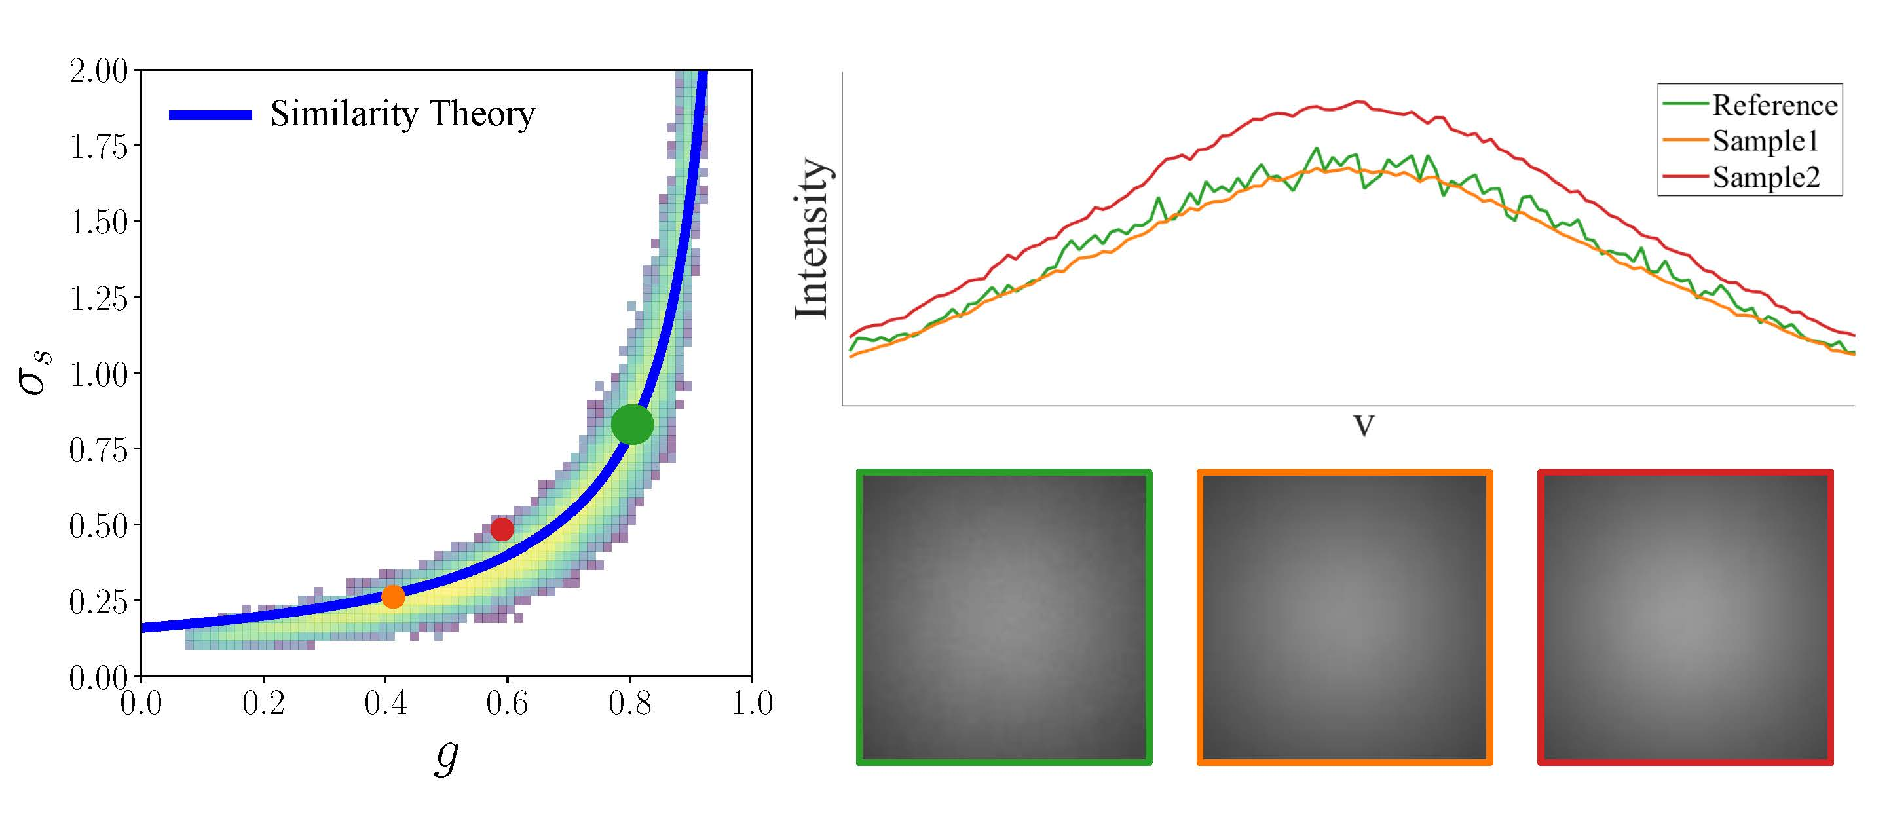
\includegraphics[width=0.98\columnwidth]{scatter/scatter.pdf}
	\end{tabular}
	\captionsetup{labelfont=bf,textfont=it}
	\caption{\label{fig:scatter}
		A motivating example of a scattering material with two estimated parameters (scattering coefficient and phase function parameter). The posterior distribution sampled with our method for three synthetic input images is able to detect the full structure of the parameter space, matching the predictions from similarity theory.
	}
\end{figure}

%\begin{figure}[t]
%	\centering
%	\addtolength{\tabcolsep}{-3pt}
%	\begin{tabular}{c}
%		\includegraphics[width=0.9\columnwidth]{images/scatter/image.png}
%	\end{tabular}
%	\caption{\label{fig:scatter2}
%	}
%\end{figure}

\subsection{Similarity Relations in Translucency}

As a motivating example, we first illustrate the behavior of the MCMC material parameter estimation process on the case of a homogeneous translucent material with two varying parameters.
In this example, the shape of the posterior can be analytically derived (using the similarity theory) and easily plotted. This serves as a demonstration and validation of our approach.

Specifically, the material parameter space of translucent materials under the radiative transfer framework~\cite{chandrasekhar1960radiative} is known to be approximately over-complete~\cite{Zhao:2014:HSR}.
Specifically, two sets of parameters $(\sigma_s, \sigma_a, g)$ and $(\sigma_s^*, \sigma_a^*, g^*)$ satisfying the following \emph{similarity relation} usually yield similar final appearances:
%
\begin{equation}
	\label{eq:similarity_rel}
	\sigma_a = \sigma_a^*, \quad (1 - g)\,\sigma_s = (1 - g^*)\,\sigma_s^*,
\end{equation}
%
where $\sigma_a$ and $\sigma_s$ are, respectively, the absorption and scattering coefficients, and $g$ is the first Legendre moment of the phase function.
We show in Figure~\ref{fig:scatter} that applying our Bayesian inference method to $\sigma_s$ and $g$ (with fixed $\sigma_a$) computes a posterior distribution that agrees well with the predicted similarity relation~\eqref{eq:similarity_rel}.

%\begin{figure*}[t]
%	\addtolength{\tabcolsep}{-4.5pt}
%	\begin{tabular}{ccccccccc}
%		& \multicolumn{2}{c}{\toptext{2\resultwidth}{Point estimate}} & \multicolumn{5}{c}{\toptext{5\resultwidth}{Bayesian inference}}\\[-4pt]
%		target & loss & optimize & posterior & sample-1 & sample-2 & sample-3& sample-4
%		\\
%		
\includegraphics[width=\resultwidth]{synth/bump/target.jpg} &
%		\includegraphics[width=\resultwidth]{synth/bump/loss.pdf} &
%		\includegraphics[width=\resultwidth]{synth/bump/optim.jpg} &
%		\includegraphics[width=\resultwidth]{synth/bump/posterior.pdf} &
%		\includegraphics[width=\resultwidth]{synth/bump/good1.jpg} &
%		\includegraphics[width=\resultwidth]{synth/bump/good2.jpg} &
%		\includegraphics[width=\resultwidth]{synth/bump/good3.jpg} &
%		\includegraphics[width=\resultwidth]{synth/bump/bad1.jpg}
%		\\
%		
\includegraphics[width=\resultwidth]{synth/leather/target.jpg} &
%		\includegraphics[width=\resultwidth]{synth/leather/loss.pdf} &
%		\includegraphics[width=\resultwidth]{synth/leather/optim.jpg} &
%		\includegraphics[width=\resultwidth]{synth/leather/posterior.pdf} &
%		\includegraphics[width=\resultwidth]{synth/leather/good1.jpg} &
%		\includegraphics[width=\resultwidth]{synth/leather/good2.jpg} &
%		\includegraphics[width=\resultwidth]{synth/leather/good3.jpg} &
%		\includegraphics[width=\resultwidth]{synth/leather/bad1.jpg}
%		\\
%		
\includegraphics[width=\resultwidth]{synth/plaster/target.jpg} &
%		\includegraphics[width=\resultwidth]{synth/plaster/loss.pdf} &
%		\includegraphics[width=\resultwidth]{synth/plaster/optim.jpg} &
%		\includegraphics[width=\resultwidth]{synth/plaster/posterior.pdf} &
%		\includegraphics[width=\resultwidth]{synth/plaster/good1.jpg} &
%		\includegraphics[width=\resultwidth]{synth/plaster/good2.jpg} &
%		\includegraphics[width=\resultwidth]{synth/plaster/good3.jpg} &
%		\includegraphics[width=\resultwidth]{synth/plaster/bad1.jpg}
%		\\
%		
\includegraphics[width=\resultwidth]{synth/flake/target.jpg} &
%		\includegraphics[width=\resultwidth]{synth/flake/loss.pdf} &
%		\includegraphics[width=\resultwidth]{synth/flake/optim.jpg} &
%		\includegraphics[width=\resultwidth]{synth/flake/posterior.pdf} &
%		\includegraphics[width=\resultwidth]{synth/flake/good1.jpg} &
%		\includegraphics[width=\resultwidth]{synth/flake/good2.jpg} &
%		\includegraphics[width=\resultwidth]{synth/flake/good3.jpg} &
%		\includegraphics[width=\resultwidth]{synth/flake/bad1.jpg}
%		\\
%		
\includegraphics[width=\resultwidth]{synth/metal/target.jpg} &
%		\includegraphics[width=\resultwidth]{synth/metal/loss.pdf} &
%		\includegraphics[width=\resultwidth]{synth/metal/optim.jpg} &
%		\includegraphics[width=\resultwidth]{synth/metal/posterior.pdf} &
%		\includegraphics[width=\resultwidth]{synth/metal/good1.jpg} &
%		\includegraphics[width=\resultwidth]{synth/metal/good2.jpg} &
%		\includegraphics[width=\resultwidth]{synth/metal/good3.jpg} &
%		\includegraphics[width=\resultwidth]{synth/metal/bad1.jpg}
%		\\
%		\includegraphics[width=\resultwidth]{synth/wood/target.jpg} &
%		\includegraphics[width=\resultwidth]{synth/wood/loss.pdf} &
%		\includegraphics[width=\resultwidth]{synth/wood/optim.jpg} &
%		\includegraphics[width=\resultwidth]{synth/wood/posterior.pdf} &
%		\includegraphics[width=\resultwidth]{synth/wood/good1.jpg} &
%		\includegraphics[width=\resultwidth]{synth/wood/good2.jpg} &
%		\includegraphics[width=\resultwidth]{synth/wood/good3.jpg} &
%		\includegraphics[width=\resultwidth]{synth/wood/bad1.jpg}
%		\\
%		& & \qquad \qquad \, low &
%		\includegraphics[width=\resultwidthpdf]{img/colorbar.jpg} &
%		high \qquad \qquad \,& & &
%	\end{tabular}
%	%
%	\caption{\label{fig:synth}
%		\textbf{Optimization and HMC sampling on synthetic images.} Each row corresponds to a different material. From top: bump, leather, plaster, metallic flake, brushed metal and wood. Column 1 is rendered images using different forward models. We show optimization results in columns 2 and 3, samplings in the rest columns. For high dimensional posterior visualization, we project them to 2D using PCA. Here we only show the first two major components. The three red dots corresponding to sample-1,2,3, which are closer to the peak of high dimensional distribution. and the green dot (sample-4) is the opposite. More results please refer to supplemental materials.
%	}
%\end{figure*}

\begin{figure*}[t]
	\centering
	\addtolength{\tabcolsep}{-4.5pt}
	\begin{tabular}{ccccccccc}
		target & sample-1 & sample-2 & sample-3 & & target & sample-1 & sample-2 & sample-3
		\\
		\begin{overpic}[width=\resultwidth]{synth/bump_1/target.jpg}
			\imglabel{Bump-1}
		\end{overpic} &
		\includegraphics[width=\resultwidth]{synth/bump_1/good1.jpg} &
		\includegraphics[width=\resultwidth]{synth/bump_1/good2.jpg} &
		\includegraphics[width=\resultwidth]{synth/bump_1/bad1.jpg} &
		&
		\begin{overpic}[width=\resultwidth]{synth/bump_2/target.jpg}
			\imglabel{Bump-2}
		\end{overpic} &
		\includegraphics[width=\resultwidth]{synth/bump_2/good1.jpg} &
		\includegraphics[width=\resultwidth]{synth/bump_2/good2.jpg} &
		\includegraphics[width=\resultwidth]{synth/bump_2/bad1.jpg}
		\\
		\begin{overpic}[width=\resultwidth]{synth/leather_1/target.jpg}
			\imglabel{Leather-1}
		\end{overpic} &
		\includegraphics[width=\resultwidth]{synth/leather_1/good1.jpg} &
		\includegraphics[width=\resultwidth]{synth/leather_1/good2.jpg} &
		\includegraphics[width=\resultwidth]{synth/leather_1/bad1.jpg} &
		&
		\begin{overpic}[width=\resultwidth]{synth/leather_2/target.jpg}
			\imglabel{Leather-2}
		\end{overpic} &
		\includegraphics[width=\resultwidth]{synth/leather_2/good1.jpg} &
		\includegraphics[width=\resultwidth]{synth/leather_2/good2.jpg} &
		\includegraphics[width=\resultwidth]{synth/leather_2/bad1.jpg}
		\\
		\begin{overpic}[width=\resultwidth]{synth/plaster_1/target.jpg}
			\imglabel{Plaster-1}
		\end{overpic} &
		\includegraphics[width=\resultwidth]{synth/plaster_1/good1.jpg} &
		\includegraphics[width=\resultwidth]{synth/plaster_1/good2.jpg} &
		\includegraphics[width=\resultwidth]{synth/plaster_1/bad1.jpg} &
		&
		\begin{overpic}[width=\resultwidth]{synth/plaster_2/target.jpg}
			\imglabel{Plaster-2}
		\end{overpic} &
		\includegraphics[width=\resultwidth]{synth/plaster_2/good1.jpg} &
		\includegraphics[width=\resultwidth]{synth/plaster_2/good2.jpg} &
		\includegraphics[width=\resultwidth]{synth/plaster_2/bad1.jpg}
		\\
		\begin{overpic}[width=\resultwidth]{synth/flake_1/target.jpg}
			\imglabel{Metallicflake-1}
		\end{overpic} &
		\includegraphics[width=\resultwidth]{synth/flake_1/good1.jpg} &
		\includegraphics[width=\resultwidth]{synth/flake_1/good2.jpg} &
		\includegraphics[width=\resultwidth]{synth/flake_1/bad1.jpg} &
		&
		\begin{overpic}[width=\resultwidth]{synth/flake_2/target.jpg}
			\imglabel{Metallicflake-2}
		\end{overpic} &
		\includegraphics[width=\resultwidth]{synth/flake_2/good1.jpg} &
		\includegraphics[width=\resultwidth]{synth/flake_2/good2.jpg} &
		\includegraphics[width=\resultwidth]{synth/flake_2/bad1.jpg}
		\\
		\begin{overpic}[width=\resultwidth]{synth/metal_1/target.jpg}
			\imglabel{Brushmetal-1}
		\end{overpic} &
		\includegraphics[width=\resultwidth]{synth/metal_1/good1.jpg} &
		\includegraphics[width=\resultwidth]{synth/metal_1/good2.jpg} &
		\includegraphics[width=\resultwidth]{synth/metal_1/bad1.jpg} &
		&
		\begin{overpic}[width=\resultwidth]{synth/metal_2/target.jpg}
			\imglabel{Brushmetal-2}
		\end{overpic} &
		\includegraphics[width=\resultwidth]{synth/metal_2/good1.jpg} &
		\includegraphics[width=\resultwidth]{synth/metal_2/good2.jpg} &
		\includegraphics[width=\resultwidth]{synth/metal_2/bad1.jpg}
		\\
		\begin{overpic}[width=\resultwidth]{synth/wood_1/target.jpg}
			\imglabel{Wood-1}
		\end{overpic} &
		\includegraphics[width=\resultwidth]{synth/wood_1/good1.jpg} &
		\includegraphics[width=\resultwidth]{synth/wood_1/good2.jpg} &
		\includegraphics[width=\resultwidth]{synth/wood_1/bad1.jpg} & &
		\begin{overpic}[width=\resultwidth]{synth/wood_2/target.jpg}
			\imglabel{Wood-2}
		\end{overpic} &
		\includegraphics[width=\resultwidth]{synth/wood_2/good1.jpg} &
		\includegraphics[width=\resultwidth]{synth/wood_2/good2.jpg} &
		\includegraphics[width=\resultwidth]{synth/wood_2/bad1.jpg}
	\end{tabular}
	\captionsetup{labelfont=bf,textfont=it}
	\caption{\label{fig:synth}
		\textbf{Results} of our MCMC sampling on \textbf{synthetic} inputs. Each row corresponds to two examples of a different material model. For each example, the first column is the synthetic target image. We show MCMC samples in the other columns, where sample-1 and sample-2 are chosen closer to the peak of the posterior distribution, and sample-3 is further away. More results please refer to supplemental materials.
	}
\end{figure*}

\begin{figure*}[t]
	\centering
	\addtolength{\tabcolsep}{-4.5pt}
	\begin{tabular}{cccccccc}
		target & sample-1 & sample-2 & sample-3 & target & sample-1 & sample-2 & sample-3
		\\
		\begin{overpic}[width=\resultwidth]{synth_discrete/leather/target.jpg}
			\imglabel{Leather-1}
		\end{overpic} &
		\includegraphics[width=\resultwidth]{synth_discrete/leather/good1.jpg} &
		\includegraphics[width=\resultwidth]{synth_discrete/leather/bad1.jpg} &
		\includegraphics[width=\resultwidth]{synth_discrete/leather/bad2.jpg} &
		\begin{overpic}[width=\resultwidth]{synth_discrete/plaster/target.jpg}
			\imglabel{Plaster-2}
		\end{overpic} &
		\includegraphics[width=\resultwidth]{synth_discrete/plaster/good1.jpg} &
		\includegraphics[width=\resultwidth]{synth_discrete/plaster/bad1.jpg} &
		\includegraphics[width=\resultwidth]{synth_discrete/plaster/bad2.jpg}
		\\
		&
		\begin{overpic}[width=\resultwidth]{synth_discrete/cell/cell_1.jpg}
			\put(0,0){\color{green}%
				\frame{\includegraphics[width=0.4\resultwidth]{synth_discrete/cell/cell_1_zoom.jpg}}}
		\end{overpic}
		&
		\begin{overpic}[width=\resultwidth]{synth_discrete/cell/cell_2.jpg}
			\put(0,0){\color{green}%
				\frame{\includegraphics[width=0.4\resultwidth]{synth_discrete/cell/cell_2_zoom.jpg}}}
		\end{overpic}
		&
		\begin{overpic}[width=\resultwidth]{synth_discrete/cell/cell_3.jpg}
			\put(0,0){\color{green}%
				\frame{\includegraphics[width=0.4\resultwidth]{synth_discrete/cell/cell_3_zoom.jpg}}}
		\end{overpic}
		&
		&
		\begin{overpic}[width=\resultwidth]{synth_discrete/noise/noise_1.jpg}
			\put(0,0){\color{green}%
				\frame{\includegraphics[width=0.4\resultwidth]{synth_discrete/noise/noise_1_zoom.jpg}}}
		\end{overpic}
		&
		\begin{overpic}[width=\resultwidth]{synth_discrete/noise/noise_2.jpg}
			\put(0,0){\color{green}%
				\frame{\includegraphics[width=0.4\resultwidth]{synth_discrete/noise/noise_2_zoom.jpg}}}
		\end{overpic}
		&
		\begin{overpic}[width=\resultwidth]{synth_discrete/noise/noise_3.jpg}
			\put(0,0){\color{green}%
				\frame{\includegraphics[width=0.4\resultwidth]{synth_discrete/noise/noise_3_zoom.jpg}}}
		\end{overpic}
		%\\
		%\multicolumn{4}{c}{(b)}
	\end{tabular}
	\captionsetup{labelfont=bf,textfont=it}
	\caption{\label{fig:discrete}
		\textbf{MCMC sampling with discrete parameters.} In these examples, we illustrate the ability of our sampling to handle discrete parameters. In both examples, one noise inputs used in the procedural model can be switched between several different types of noise. Out of the thousands of sampled solutions, we pick three that have different settings of the discrete parameter where the (log) pdf values decrease from sample-1 to sample-3.
	}
\end{figure*}

\begin{figure*}[t]
	\centering
	\addtolength{\tabcolsep}{-4.5pt}
	\begin{tabular}{ccccccccc}
		photo & sample-1 & sample-2 & sample-3 & & photo & sample-1 & sample-2 & sample-3
		\\
		\begin{overpic}[width=\resultwidth]{images/real/bump3/out/target.png}
			\imglabel{Bump-3}
		\end{overpic} &
		\includegraphics[width=\resultwidth]{images/real/bump3/out/good1.png} &
		\includegraphics[width=\resultwidth]{images/real/bump3/out/good2.png} &
		\includegraphics[width=\resultwidth]{images/real/bump3/out/bad1.png} &
		&
		\begin{overpic}[width=\resultwidth]{images/real/bump2/out/target.png}
			\imglabel{Bump-4}
		\end{overpic} &
		\includegraphics[width=\resultwidth]{images/real/bump2/out/good1.png} &
		\includegraphics[width=\resultwidth]{images/real/bump2/out/good2.png} &
		\includegraphics[width=\resultwidth]{images/real/bump2/out/bad1.png}
		\\
		\begin{overpic}[width=\resultwidth]{images/real/leather/out/target.jpg}
			\imglabel{Leather-3}
		\end{overpic} &
		\includegraphics[width=\resultwidth]{images/real/leather/out/good1.jpg} &
		\includegraphics[width=\resultwidth]{images/real/leather/out/good2.jpg} &
		\includegraphics[width=\resultwidth]{images/real/leather/out/bad1.jpg} &
		&
		\begin{overpic}[width=\resultwidth]{images/real/leather2/out/target.png}
			\imglabel{Leather-4}
		\end{overpic} &
		\includegraphics[width=\resultwidth]{images/real/leather2/out/good1.png} &
		\includegraphics[width=\resultwidth]{images/real/leather2/out/good2.png} &
		\includegraphics[width=\resultwidth]{images/real/leather2/out/bad1.png}
		\\
		\begin{overpic}[width=\resultwidth]{images/real/leather3/out/target.png}
			\imglabel{Leather-5}
		\end{overpic} &
		\includegraphics[width=\resultwidth]{images/real/leather3/out/good1.png} &
		\includegraphics[width=\resultwidth]{images/real/leather3/out/good2.png} &
		\includegraphics[width=\resultwidth]{images/real/leather3/out/bad1.png} &
		&
		\begin{overpic}[width=\resultwidth]{images/real/leather4/out/target.png}
			\imglabel{Leather-6}
		\end{overpic} &
		\includegraphics[width=\resultwidth]{images/real/leather4/out/good1.png} &
		\includegraphics[width=\resultwidth]{images/real/leather4/out/good2.png} &
		\includegraphics[width=\resultwidth]{images/real/leather4/out/bad1.png}
		\\
		\begin{overpic}[width=\resultwidth]{images/real/plaster/out/target.jpg}
			\imglabel{Plaster-3}
		\end{overpic} &
		\includegraphics[width=\resultwidth]{images/real/plaster/out/good1.jpg} &
		\includegraphics[width=\resultwidth]{images/real/plaster/out/good2.jpg} &
		\includegraphics[width=\resultwidth]{images/real/plaster/out/bad1.jpg} &
		&
		\begin{overpic}[width=\resultwidth]{images/real/plaster2/out/target.png}
			\imglabel{Plaster-4}
		\end{overpic} &
		\includegraphics[width=\resultwidth]{images/real/plaster2/out/good1.png} &
		\includegraphics[width=\resultwidth]{images/real/plaster2/out/good2.png} &
		\includegraphics[width=\resultwidth]{images/real/plaster2/out/bad1.png}
		\\
		\begin{overpic}[width=\resultwidth]{images/real/flake/out/target.jpg}
			\imglabel{Metallicflake-3}
		\end{overpic} &
		\includegraphics[width=\resultwidth]{images/real/flake/out/good1.jpg} &
		\includegraphics[width=\resultwidth]{images/real/flake/out/good2.jpg} &
		\includegraphics[width=\resultwidth]{images/real/flake/out/bad1.jpg} &
		&
		\begin{overpic}[width=\resultwidth]{images/real/flake2/out/target.png}
			\imglabel{Metallicflake-4}
		\end{overpic} &
		\includegraphics[width=\resultwidth]{images/real/flake2/out/good1.png} &
		\includegraphics[width=\resultwidth]{images/real/flake2/out/good2.png} &
		\includegraphics[width=\resultwidth]{images/real/flake2/out/bad1.png}
		\\
		\begin{overpic}[width=\resultwidth]{images/real/metal/out/target.png}
			\imglabel{Brushmetal-3}
		\end{overpic} &
		\includegraphics[width=\resultwidth]{images/real/metal/out/good1.png} &
		\includegraphics[width=\resultwidth]{images/real/metal/out/good2.png} &
		\includegraphics[width=\resultwidth]{images/real/metal/out/bad1.png} &
		&
		\begin{overpic}[width=\resultwidth]{images/real/wood/out/target.jpg}
			\imglabel{Wood-3}
		\end{overpic} &
		\includegraphics[width=\resultwidth]{images/real/wood/out/good1.jpg} &
		\includegraphics[width=\resultwidth]{images/real/wood/out/good2.jpg} &
		\includegraphics[width=\resultwidth]{images/real/wood/out/bad1.jpg}
		\\
		\begin{overpic}[width=\resultwidth]{images/real/wood2/out/target.png}
			\imglabel{Wood-4}
		\end{overpic} &
		\includegraphics[width=\resultwidth]{images/real/wood2/out/good1.png} &
		\includegraphics[width=\resultwidth]{images/real/wood2/out/good2.png} &
		\includegraphics[width=\resultwidth]{images/real/wood2/out/bad1.png} &
		&
		\begin{overpic}[width=\resultwidth]{images/real/wood3/out/target.png}
			\imglabel{Wood-5}
		\end{overpic} &
		\includegraphics[width=\resultwidth]{images/real/wood3/out/good1.png} &
		\includegraphics[width=\resultwidth]{images/real/wood3/out/good2.png} &
		\includegraphics[width=\resultwidth]{images/real/wood3/out/bad1.png}
	\end{tabular}
	\caption{\label{fig:real}
		Results of our MCMC sampling on \textbf{real} inputs. For each example, the first column is the real target image (photo). We show MCMC samples in the other columns, where sample-1 and sample-2 are chosen closer to the peak of the posterior distribution, and sample-3 is further away. Note that the target images for Plaster-4 and Wood-5 are captured under natural illumination, while the corresponding synthetic images still assume collocated flash illumination; despite this mismatch, the estimated material parameters are still reasonable. Note, target images for Leather-4, Leather-6 and Wood-4 are from the publicly released dataset of \cite{Aittala2016}. For more results please refer to supplemental materials.
	}
\end{figure*}

\begin{table}[t]
	\centering
	\caption{\label{fig:performance}
		%\sz{Need to be updated if we used MALA.}
		Performance statistics for our MCMC-based posterior sampling.
		The numbers are collected using a workstation equipped with an Intel i7-6800K six-core CPU and an Nvidia GTX 1080 GPU.  %\protect\footnotemark.
	}
%	\begin{tabular}{l|c|c}
%		\multirow{2}{*}{\textbf{Material}} & \multirow{2}{*}{\textbf{\# params}} & {\textbf{MCMC}}\\
%		& & (1k iter.)\\
%		\hline
%		Bump    &  8 & 180 s\\
%		Leather & 12 & 194 s\\
%		Plaster & 11 & 190 s\\
%		Flakes  & 13 & 187 s\\
%		Metal   & 10 & 182 s\\
%		Wood    & 23 & 290 s
%	\end{tabular}
	\addtolength{\tabcolsep}{-3pt}
	\begin{tabular}{l|rrrrrr}
		\textbf{Material} & bump & leather & plaster & flakes & metal & wood\\
		\hline
		\textbf{\# params.} & 8 & 12 & 11 & 13 & 10 & 23\\
		\textbf{MCMC} (1k iter.) & 180 s & 194 s & 190 s & 187 s & 182 s & 290 s
	\end{tabular}
\end{table}

%\footnotetext{In HMC sampling, each sample needs $(s+3)/r$ forward evaluations on average where $s$ indicates the number of leapfrog steps and $r$ denotes the acceptance rate. In practice, we set $s = 4$ and have $r = 70\%$, causing the expected number of evaluations per sample to be 10.}


\subsection{Procedural Material  Models}
\label{ssec:proc_models}
%
We show results generated using synthetic images in Figures~\ref{fig:synth} and \ref{fig:discrete} as well as real photographs (taken with different cameras) in Figure~\ref{fig:real}.
%The captions of the figures provide more detail.
Please see the supplemental material for more results, including animations illustrating point estimations and sampling. Below we describe the six procedural models tested. Please refer to the supplement for additional detail and a PyTorch implementation. For each parameter, we define a reasonable truncated Gaussian distribution as its prior (also see supplement). In most cases, the MCMC sampling starts from the peak of the prior. In some examples (e.g wood), we first run posterior maximization and then switch to sampling from the optimized point. We drop some number (typically 200 to 1000) of initial MCMC samples due to burn-in.

\paragraph*{Bumpy microfacet surface.}
This model depicts an opaque dielectric surface with an isotropic noise heightfield. We use a standard microfacet BRDF with the GGX normal distribution~\cite{Walter2007} combined with a normal map computed from an explicitly constructed heightfield. We assume that the Fresnel reflectance at normal incidence can be computed from a known index of refraction (a value of 1.5 is a good estimate for plastics). We assume an unknown roughness $r$ (GGX parameter $\alpha=r^2$) and a Lambertian diffuse term with unknown albedo $\rho$. This model is identical to Wang et al.~\cite{Wang2011}, except using the GGX instead of Beckmann microfacet distribution. The main practical difference from the capture setup in that paper is that we use a point light, instead of step-edge illumination.

The bumpy heightfield is constructed using an inverse Fourier process including: (i)~choosing a power spectrum in the continuous Fourier domain; (ii)~discretizing it onto a grid of complex numbers; (iii)~randomly choosing the phase of each texel on the grid (while keeping the chosen amplitude); and (iv)~applying an inverse fast Fourier transform whose
real component becomes the resulting heightfield.
At render time, we use the normal map derived from this heightfield.
%The normal map can be computed from the heightfield (finite differences work well).

\paragraph*{Leather and plaster.}
These materials can be modeled similarly as the aforementioned bumpy surfaces except for the computation of the heightfield and roughness.
For plaster, a fractal noise texture is scaled (in space and intensity) and thresholded (controlled by additional parameters) to produce both the heightfield and a roughness variation texture. For leather, on the contrary, a Voronoi cell map is used to get the effect of leather-like cells (with parameters for scaling and thresholding), and additional small-scale fractal noise is added.
Further, we use multiple (pre-generated) noise textures and Voronoi cell maps to diversify the micro-scale appearances that our models can produce.
The choice of these textures and maps is captured using a discrete parameter.
In Figure~\ref{fig:discrete}, we show a few example samples drawn from the posterior distributions using Algorithm~\ref{alg:mcmc_sample}.

\paragraph*{Brushed metal.} The brushed metal material extends the above bumpy surface, by introducing anisotropy to both the GGX normal distribution and the noise heightfield used to compute the normal map, while dropping the diffuse term. We make both the BRDF and the Fourier-domain Gaussian power spectrum anisotropic. The parameters of the model thus include two roughnesses, as well as two Fourier-domain standard deviations.  We make the anisotropic highlight vertical and centered in the target image.

\paragraph*{Metallic flakes.} Metallic paint with flakes is a stochastic material with multiple BRDF lobes (caused by light reflecting off the flakes). Our model involves three components, each being an isotropic microfacet lobe, to describe top coating, flakes and glow, respectively. The top coating is usually highly specular, and we make its roughness a model parameter. We assume an index of refraction of 1.5, implying a Fresnel (Schlick) reflectivity at normal incidence of 0.04. The flakes are chosen as Voronoi cells of a random blue-noise point distribution; they have a roughness parameter and varying normals chosen from the Beckmann distribution with an unknown roughness, and with unknown Fresnel reflectivity. The scale of the cell map is itself a (differentiable) parameter. Lastly, the glow is a component approximating the internal scattering between the top interface and the flakes, and has its own roughness, Fresnel reflectivity and a flat normal. An extra weight parameter linearly combines the flakes and the glow.

\paragraph*{Wood.} Lastly, we created a partial PyTorch implementation of the comprehensive 3D wood model of Liu et al.~\cite{Liu2016}. This material is a 3D model of the growth rings of a tree, with a number of parameters controlling colors and widths of growth rings, as well as global distortions and small-scale noise features. The 3D wood is finally projected by a cutting plane to image space, defining diffuse albedo, roughness and height.

\section{Conclusion}

We have introduced a framework parameter estimation for globally parameterized material models with various optical properties (bumpy paint, metallic paint, scattering medium with Fresnel interface, brushed metal). For each of these, we introduced a differentiable forward evaluator, implemented using \torch.

We proposed several \emph{summary functions}, enabling us to compare a synthetic simulation image to a target image (photo) effectively, by comparing their summary vectors; comparing them directly would not be feasible, as we cannot assume per-pixel match between the features.

Finally, we introduced Bayesian inference through Hamiltonian Monte Carlo sampling of the posterior distribution of material parameters. This allows us to resolve \emph{similarity structures} (areas of almost equally good fit) in the material parameter spaces. This lets us handle models with a highly non-linear parameterization, obtaining good appearance matches from a single photograph.

Because our material models are global instead of based on textures of per-pixel parameters, they can cover large areas without repetition, can be easily edited, and require minimal storage. In the future, we would like increase the complexity of the models supported even further, to handle materials like woven fabrics, transmissive BTDFs, and more.


\bibliographystyle{ACM-Reference-Format}
\bibliography{references}

%\input{appendix}
%\newpage
\section{Supplemental images}
\label{sec:supp}
%
% \subsection{Bumpy surface}
% Motivation: Four images below are pixel-wise different. But from human perception, we consider the images in each row are equivalent.

% \begin{figure}[H]
% 	\addtolength{\tabcolsep}{-3.5pt}
% 	\begin{tabular}{ccc}
% 		\includegraphics[width=0.30\columnwidth]{results/bump/syn_comp/bump04rd1.png} &
% 		\includegraphics[width=0.30\columnwidth]{results/bump/syn_comp/bump04rd2.png} &
% 		\includegraphics[width=0.35\columnwidth]{results/bump/syn_comp/bump04diff.pdf} \\
% 		\includegraphics[width=0.30\columnwidth]{results/bump/syn_comp/bump02rd1.png} &
% 		\includegraphics[width=0.30\columnwidth]{results/bump/syn_comp/bump02rd2.png} &
% 		\includegraphics[width=0.35\columnwidth]{results/bump/syn_comp/bump02diff.pdf} \\
% 	\end{tabular}
% 	\caption{\label{fig:syn1}
% 		Two images in each row have same parameters but with different randomness. The images in bottom row have smoother brdf.
% 	}
% \end{figure}


\newpage
\subsubsection{Synthetic data}
XXXXXXXXXX

\begin{figure}[H]
	\includegraphics[width=0.4\columnwidth]{results/bump/syn_comp/bump02rd1.png}
	\caption{
		Target image (reference)
	}
\end{figure}


\begin{figure}[H]
	\addtolength{\tabcolsep}{-3.5pt}
	\begin{tabular}{ccc}
		\includegraphics[width=0.30\columnwidth]{results/bump/syn0/rd.png} &
		\includegraphics[width=0.30\columnwidth]{results/bump/syn0/rd1.png} &
		\includegraphics[width=0.30\columnwidth]{results/bump/syn0/rd2.png} \\
		\includegraphics[width=0.30\columnwidth]{results/bump/syn0/rd3.png} &
		\includegraphics[width=0.30\columnwidth]{results/bump/syn0/rd4.png} &
		\includegraphics[width=0.30\columnwidth]{results/bump/syn0/rd5.png} \\
		\includegraphics[width=0.30\columnwidth]{results/bump/syn0/rd6.png} &
		\includegraphics[width=0.30\columnwidth]{results/bump/syn0/rd7.png} &
		\includegraphics[width=0.30\columnwidth]{results/bump/syn0/rd8.png} \\
	\end{tabular}
	\caption{
		Random picked from HMC sampled results. Only use mean.
	}
\end{figure}

\begin{figure}[H]
	\addtolength{\tabcolsep}{-3.5pt}
	\begin{tabular}{ccc}
		\includegraphics[width=0.30\columnwidth]{results/bump/syn0/rd.pdf} &
		\includegraphics[width=0.30\columnwidth]{results/bump/syn0/rd1.pdf} &
		\includegraphics[width=0.30\columnwidth]{results/bump/syn0/rd2.pdf} \\
		\includegraphics[width=0.30\columnwidth]{results/bump/syn0/rd3.pdf} &
		\includegraphics[width=0.30\columnwidth]{results/bump/syn0/rd4.pdf} &
		\includegraphics[width=0.30\columnwidth]{results/bump/syn0/rd5.pdf} \\
		\includegraphics[width=0.30\columnwidth]{results/bump/syn0/rd6.pdf} &
		\includegraphics[width=0.30\columnwidth]{results/bump/syn0/rd7.pdf} &
		\includegraphics[width=0.30\columnwidth]{results/bump/syn0/rd8.pdf} \\
	\end{tabular}
	\caption{
		Corresponding posterior and picked point. Only use mean.
	}
\end{figure}



\begin{figure}[H]
	\addtolength{\tabcolsep}{-3.5pt}
	\begin{tabular}{ccc}
		\includegraphics[width=0.30\columnwidth]{results/bump/syn1/rd.png} &
		\includegraphics[width=0.30\columnwidth]{results/bump/syn1/rd1.png} &
		\includegraphics[width=0.30\columnwidth]{results/bump/syn1/rd2.png} \\
		\includegraphics[width=0.30\columnwidth]{results/bump/syn1/rd3.png} &
		\includegraphics[width=0.30\columnwidth]{results/bump/syn1/rd4.png} &
		\includegraphics[width=0.30\columnwidth]{results/bump/syn1/rd5.png} \\
		\includegraphics[width=0.30\columnwidth]{results/bump/syn1/rd6.png} &
		\includegraphics[width=0.30\columnwidth]{results/bump/syn1/rd7.png} &
		\includegraphics[width=0.30\columnwidth]{results/bump/syn1/rd8.png} \\
	\end{tabular}
	\caption{
		Random picked from HMC sampled results. Use mean and stddev.
	}
\end{figure}

\begin{figure}[H]
	\addtolength{\tabcolsep}{-3.5pt}
	\begin{tabular}{ccc}
		\includegraphics[width=0.30\columnwidth]{results/bump/syn1/rd.pdf} &
		\includegraphics[width=0.30\columnwidth]{results/bump/syn1/rd1.pdf} &
		\includegraphics[width=0.30\columnwidth]{results/bump/syn1/rd2.pdf} \\
		\includegraphics[width=0.30\columnwidth]{results/bump/syn1/rd3.pdf} &
		\includegraphics[width=0.30\columnwidth]{results/bump/syn1/rd4.pdf} &
		\includegraphics[width=0.30\columnwidth]{results/bump/syn1/rd5.pdf} \\
		\includegraphics[width=0.30\columnwidth]{results/bump/syn1/rd6.pdf} &
		\includegraphics[width=0.30\columnwidth]{results/bump/syn1/rd7.pdf} &
		\includegraphics[width=0.30\columnwidth]{results/bump/syn1/rd8.pdf} \\
	\end{tabular}
	\caption{
		Corresponding posterior and picked point. Use mean and stddev.
	}
\end{figure}

\begin{figure}[H]
	\includegraphics[width=0.7\columnwidth]{placeholder/placeholder.jpg}
	\caption{
		PLACEHOLDER
	}
\end{figure}


\begin{figure}[H]
	\addtolength{\tabcolsep}{-3.5pt}
	\begin{tabular}{ccc}
		\includegraphics[width=0.30\columnwidth]{results/bump/syn2/rd.png} &
		\includegraphics[width=0.30\columnwidth]{results/bump/syn2/rd1.png} &
		\includegraphics[width=0.30\columnwidth]{results/bump/syn2/rd2.png} \\
		\includegraphics[width=0.30\columnwidth]{results/bump/syn2/rd3.png} &
		\includegraphics[width=0.30\columnwidth]{results/bump/syn2/rd4.png} &
		\includegraphics[width=0.30\columnwidth]{results/bump/syn2/rd5.png} \\
		\includegraphics[width=0.30\columnwidth]{results/bump/syn2/rd6.png} &
		\includegraphics[width=0.30\columnwidth]{results/bump/syn2/rd7.png} &
		\includegraphics[width=0.30\columnwidth]{results/bump/syn2/rd8.png} \\
	\end{tabular}
	\caption{
		Random picked from HMC sampled results. Use mean and 2D FFT.
	}
\end{figure}

\begin{figure}[H]
	\addtolength{\tabcolsep}{-3.5pt}
	\begin{tabular}{ccc}
		\includegraphics[width=0.30\columnwidth]{results/bump/syn2/rd.pdf} &
		\includegraphics[width=0.30\columnwidth]{results/bump/syn2/rd1.pdf} &
		\includegraphics[width=0.30\columnwidth]{results/bump/syn2/rd2.pdf} \\
		\includegraphics[width=0.30\columnwidth]{results/bump/syn2/rd3.pdf} &
		\includegraphics[width=0.30\columnwidth]{results/bump/syn2/rd4.pdf} &
		\includegraphics[width=0.30\columnwidth]{results/bump/syn2/rd5.pdf} \\
		\includegraphics[width=0.30\columnwidth]{results/bump/syn2/rd6.pdf} &
		\includegraphics[width=0.30\columnwidth]{results/bump/syn2/rd7.pdf} &
		\includegraphics[width=0.30\columnwidth]{results/bump/syn2/rd8.pdf} \\
	\end{tabular}
	\caption{
		Corresponding posterior and picked point. Use mean and 2D FFT.
	}
\end{figure}

\begin{figure}[H]
	\includegraphics[width=0.7\columnwidth]{placeholder/placeholder.jpg}
	\caption{
		PLACEHOLDER
	}
\end{figure}

\subsubsection{Real photo}
XXXXXXXXXX

\begin{figure}[H]
	\includegraphics[width=0.45\columnwidth]{results/bump/real1/target.png}
	\caption{
		Target image (reference)
	}
\end{figure}


\begin{figure}[H]
	\addtolength{\tabcolsep}{-3.5pt}
	\begin{tabular}{ccc}
		\includegraphics[width=0.30\columnwidth]{results/bump/real1/rd.png} &
		\includegraphics[width=0.30\columnwidth]{results/bump/real1/rd1.png} &
		\includegraphics[width=0.30\columnwidth]{results/bump/real1/rd2.png} \\
		\includegraphics[width=0.30\columnwidth]{results/bump/real1/rd3.png} &
		\includegraphics[width=0.30\columnwidth]{results/bump/real1/rd4.png} &
		\includegraphics[width=0.30\columnwidth]{results/bump/real1/rd5.png} \\
		\includegraphics[width=0.30\columnwidth]{results/bump/real1/rd6.png} &
		\includegraphics[width=0.30\columnwidth]{results/bump/real1/rd7.png} &
		\includegraphics[width=0.30\columnwidth]{results/bump/real1/rd8.png} \\
	\end{tabular}
	\caption{
		Random picked from HMC sampled results. Use image mean and fft mean.
	}
\end{figure}

\begin{figure}[H]
	\addtolength{\tabcolsep}{-3.5pt}
	\begin{tabular}{ccc}
		\includegraphics[width=0.30\columnwidth]{results/bump/real1/rd.pdf} &
		\includegraphics[width=0.30\columnwidth]{results/bump/real1/rd1.pdf} &
		\includegraphics[width=0.30\columnwidth]{results/bump/real1/rd2.pdf} \\
		\includegraphics[width=0.30\columnwidth]{results/bump/real1/rd3.pdf} &
		\includegraphics[width=0.30\columnwidth]{results/bump/real1/rd4.pdf} &
		\includegraphics[width=0.30\columnwidth]{results/bump/real1/rd5.pdf} \\
		\includegraphics[width=0.30\columnwidth]{results/bump/real1/rd6.pdf} &
		\includegraphics[width=0.30\columnwidth]{results/bump/real1/rd7.pdf} &
		\includegraphics[width=0.30\columnwidth]{results/bump/real1/rd8.pdf} \\
	\end{tabular}
	\caption{
		Corresponding posterior and picked point. Use image mean and fft mean.
	}
\end{figure}



\subsection{Brushed metal}

\subsubsection{Real photo}
XXXXXXXXXX

\begin{figure}[H]
	\includegraphics[width=0.4\columnwidth]{results/brushed/real1/target.png}
	\caption{
		Target image (reference)
	}
\end{figure}


\begin{figure}[H]
	\addtolength{\tabcolsep}{-3.5pt}
	\begin{tabular}{ccc}
		\includegraphics[width=0.30\columnwidth]{results/brushed/real1/rd.png} &
		\includegraphics[width=0.30\columnwidth]{results/brushed/real1/rd1.png} &
		\includegraphics[width=0.30\columnwidth]{results/brushed/real1/rd2.png} \\
		\includegraphics[width=0.30\columnwidth]{results/brushed/real1/rd3.png} &
		\includegraphics[width=0.30\columnwidth]{results/brushed/real1/rd4.png} &
		\includegraphics[width=0.30\columnwidth]{results/brushed/real1/rd5.png} \\
		\includegraphics[width=0.30\columnwidth]{results/brushed/real1/rd6.png} &
		\includegraphics[width=0.30\columnwidth]{results/brushed/real1/rd7.png} &
		\includegraphics[width=0.30\columnwidth]{results/brushed/real1/rd8.png} \\
	\end{tabular}
	\caption{
		Random picked from HMC sampled results. Use image mean and fft mean.
	}
\end{figure}

\begin{figure}[H]
	\addtolength{\tabcolsep}{-3.5pt}
	\begin{tabular}{ccc}
		\includegraphics[width=0.30\columnwidth,height=0.15\columnwidth]{results/brushed/real1/rd.pdf} &
		\includegraphics[width=0.30\columnwidth,height=0.15\columnwidth]{results/brushed/real1/rd1.pdf} &
		\includegraphics[width=0.30\columnwidth,height=0.15\columnwidth]{results/brushed/real1/rd2.pdf} \\
		\includegraphics[width=0.30\columnwidth,height=0.15\columnwidth]{results/brushed/real1/rd3.pdf} &
		\includegraphics[width=0.30\columnwidth,height=0.15\columnwidth]{results/brushed/real1/rd4.pdf} &
		\includegraphics[width=0.30\columnwidth,height=0.15\columnwidth]{results/brushed/real1/rd5.pdf} \\
		\includegraphics[width=0.30\columnwidth,height=0.15\columnwidth]{results/brushed/real1/rd6.pdf} &
		\includegraphics[width=0.30\columnwidth,height=0.15\columnwidth]{results/brushed/real1/rd7.pdf} &
		\includegraphics[width=0.30\columnwidth,height=0.15\columnwidth]{results/brushed/real1/rd8.pdf} \\
	\end{tabular}
	\caption{
		Corresponding posterior and picked point. Use image mean and fft mean.
	}
\end{figure}

\subsection{Metallic flakes}

\subsubsection{Synthetic data}
XXXXXXXXXX

\begin{figure}[H]
	\includegraphics[width=0.45\columnwidth]{results/flake/syn1/target.png}
	\caption{
		Target image (reference)
	}
\end{figure}

\begin{figure}[H]
	\addtolength{\tabcolsep}{-3.5pt}
	\begin{tabular}{ccc}
		\includegraphics[width=0.30\columnwidth]{results/flake/syn1/rd0.png} &
		\includegraphics[width=0.30\columnwidth]{results/flake/syn1/rd1.png} &
		\includegraphics[width=0.30\columnwidth]{results/flake/syn1/rd2.png} \\
		\includegraphics[width=0.30\columnwidth]{results/flake/syn1/rd3.png} &
		\includegraphics[width=0.30\columnwidth]{results/flake/syn1/rd4.png} &
		\includegraphics[width=0.30\columnwidth]{results/flake/syn1/rd5.png} \\
		\includegraphics[width=0.30\columnwidth]{results/flake/syn1/rd6.png} &
		\includegraphics[width=0.30\columnwidth]{results/flake/syn1/rd7.png} &
		\includegraphics[width=0.30\columnwidth]{results/flake/syn1/rd8.png} \\
	\end{tabular}
	\caption{
		Random picked from HMC sampled results.
	}
\end{figure}

\begin{figure}[H]
	\addtolength{\tabcolsep}{-3.5pt}
	\begin{tabular}{ccc}
		\includegraphics[width=0.30\columnwidth]{results/flake/syn1/rd0.pdf} &
		\includegraphics[width=0.30\columnwidth]{results/flake/syn1/rd1.pdf} &
		\includegraphics[width=0.30\columnwidth]{results/flake/syn1/rd2.pdf} \\
		\includegraphics[width=0.30\columnwidth]{results/flake/syn1/rd3.pdf} &
		\includegraphics[width=0.30\columnwidth]{results/flake/syn1/rd4.pdf} &
		\includegraphics[width=0.30\columnwidth]{results/flake/syn1/rd5.pdf} \\
		\includegraphics[width=0.30\columnwidth]{results/flake/syn1/rd6.pdf} &
		\includegraphics[width=0.30\columnwidth]{results/flake/syn1/rd7.pdf} &
		\includegraphics[width=0.30\columnwidth]{results/flake/syn1/rd8.pdf} \\
	\end{tabular}
	\caption{
		Corresponding posterior and picked point.
	}
\end{figure}

\subsubsection{Real photo}
XXXXXXXXXX

\begin{figure}[H]
	\includegraphics[width=0.45\columnwidth]{results/flake/real1/target.png}
	\caption{
		Target image (reference)
	}
\end{figure}

\begin{figure}[H]
	\addtolength{\tabcolsep}{-3.5pt}
	\begin{tabular}{ccc}
		\includegraphics[width=0.30\columnwidth]{results/flake/real1/rd.png} &
		\includegraphics[width=0.30\columnwidth]{results/flake/real1/rd1.png} &
		\includegraphics[width=0.30\columnwidth]{results/flake/real1/rd2.png} \\
		\includegraphics[width=0.30\columnwidth]{results/flake/real1/rd3.png} &
		\includegraphics[width=0.30\columnwidth]{results/flake/real1/rd4.png} &
		\includegraphics[width=0.30\columnwidth]{results/flake/real1/rd5.png} \\
		\includegraphics[width=0.30\columnwidth]{results/flake/real1/rd6.png} &
		\includegraphics[width=0.30\columnwidth]{results/flake/real1/rd7.png} &
		\includegraphics[width=0.30\columnwidth]{results/flake/real1/rd8.png} \\
	\end{tabular}
	\caption{
		Random picked from HMC sampled results.
	}
\end{figure}

\begin{figure}[H]
	\addtolength{\tabcolsep}{-3.5pt}
	\begin{tabular}{ccc}
		\includegraphics[width=0.30\columnwidth]{results/flake/real1/rd.pdf} &
		\includegraphics[width=0.30\columnwidth]{results/flake/real1/rd1.pdf} &
		\includegraphics[width=0.30\columnwidth]{results/flake/real1/rd2.pdf} \\
		\includegraphics[width=0.30\columnwidth]{results/flake/real1/rd3.pdf} &
		\includegraphics[width=0.30\columnwidth]{results/flake/real1/rd4.pdf} &
		\includegraphics[width=0.30\columnwidth]{results/flake/real1/rd5.pdf} \\
		\includegraphics[width=0.30\columnwidth]{results/flake/real1/rd6.pdf} &
		\includegraphics[width=0.30\columnwidth]{results/flake/real1/rd7.pdf} &
		\includegraphics[width=0.30\columnwidth]{results/flake/real1/rd8.pdf} \\
	\end{tabular}
	\caption{
		Corresponding posterior and picked point.
	}
\end{figure}

\subsection{Scattering medium}

\begin{figure}[H]
	\includegraphics[width=0.95\columnwidth]{results/scatter/synthetic1/image.png}
	\caption{
		In this example, first we want to show that the similarity theory curve is properly covered by our sampled posterior. Secondly, if two points on the similarity curve are not close to each other, the rendered results have 20 percent mismatch around the peak. But in our method, we can easily find a better match.
	}
\end{figure}
%In Figures~\ref{fig:a}




\end{document}
